\documentclass{beamer}

\usetheme{Warsaw}

\title{Uppaal. The Model Checker.}
\author{Patryk Kiepas}
\date{\today}

\begin{document}
%-------------------------------------------------------------------------
\begin{frame}
	\titlepage
\end{frame}

%-------------------------------------------------------------------------	
\section*{Outline}
\begin{frame}
	\tableofcontents
\end{frame}

%%%%%%%%%%%%%%%%%%%%%%%%%%%%%%%%%%%%%%%%%%%%%%%%%%%%%%%%%%%%%%%%%%%%%%%%%%
\section{Intro}
%%%%%%%%%%%%%%%%%%%%%%%%%%%%%%%%%%%%%%%%%%%%%%%%%%%%%%%%%%%%%%%%%%%%%%%%%%
\subsection{Quick look}
%-------------------------------------------------------------------------
\begin{frame}{Uppaal. What is it?}
	Uppaal is a model checker for real-time systems (in mind of embedded systems). What we can do with it?
	
	\begin{enumerate}
		\item Modeling
		\item Simulation
		\item Verification
	\end{enumerate}
	
	Internal representation of model consists of:
	
	\begin{itemize}
		\item Network of timed automata
		\item Extended with data types
	\end{itemize}

\end{frame}

\begin{frame}{Where to use?}
	``Any system can be analysed using a model checker, as long as it has \textit{states} and \textit{transitions} between states'' (from Chapter 1: A First Introduction to Uppaal by Frits Vaandrager) \newline
	
	Reactive systems such as:
	\begin{itemize}
		\item Hardware components
		\item Embedded controllers
		\item Network protocols
		\item Others...
	\end{itemize}
	Whenever there is need to handle real-time issues (the timing of transitions).
	
\end{frame}

\subsection{History}
%-------------------------------------------------------------------------
\begin{frame}{Brief history}
	Uppaal was started by Uppsala University, Sweden and Aalborg University, Denmark.
	
	Time-line of development:
	\begin{itemize}
		\item 1995 - project started
		\item 1999 - first beta
		\item 1999/2000 - first stable release (v 3.0.X)
		\item September 27, 2010 - latest stable release (v 4.0.13)
		\item July 1, 2014 - preview release (v 4.1.19)
	\end{itemize}
	
\end{frame}

\subsection{Versions}
\begin{frame}{Uppaal variations}
	Versions: Windows, Mac, Linux, 32/64 bits
	
	Available licenses:
	\begin{itemize}
		\item Academic use (more info: \href{http://www.uppaal.org/}{http://www.uppaal.org/})
		\item Commercial use (more info: \href{http://www.uppaal.com/}{http://www.uppaal.com/})
	\end{itemize}
	
	Uppaal GUI was programmed in Java, and Uppaal checking engine was developed using C++.
\end{frame}

\begin{frame}{Extensions}
	
	\begin{itemize}
		\item \textbf{Cora} - Cost Optimal Reachability Analysis;
		\item \textbf{Tron} - Testing Real-time systems ON-line (black-box conformance testing);
		\item \textbf{Cover} - COVERerage-optimal off-line test generation;
		\item \textbf{Tiga} - TImed GAmes based controller synthesis;
		\item \textbf{Port} - component based timed systems, exploiting Partial Order Reduction Techniques;
		\item \textbf{Pro} - PRObabilistic reachability analysis;
		\item \textbf{Times} - A Tool for Modelling and Implementation of Embedded Systems;
		\item \textbf{Stratego} - Strategy synthesis, learning, optimization and evaluation;
		\item \textbf{SMC} - Statistical Model-Checker.
	\end{itemize}
	
\end{frame}

%%%%%%%%%%%%%%%%%%%%%%%%%%%%%%%%%%%%%%%%%%%%%%%%%%%%%%%%%%%%%%%%%%%%%%%%%%	
\section{The tool}
%%%%%%%%%%%%%%%%%%%%%%%%%%%%%%%%%%%%%%%%%%%%%%%%%%%%%%%%%%%%%%%%%%%%%%%%%%
\subsection{Uppaal GUI}
%%%%%%%%%%%%%%%%%%%%%%%%%%%%%%%%%%%%%%%%%%%%%%%%%%%%%%%%%%%%%%%%%%%%%%%%%%
\begin{frame}{Uppaal GUI - Main parts}
\vspace{-10mm}
\begin{columns}
	\begin{column}{0.8\textwidth}
		\begin{figure}[H]
			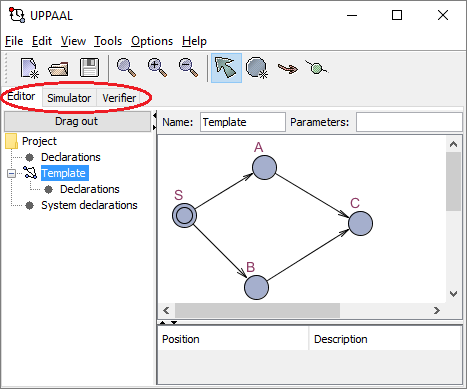
\includegraphics[scale=0.7]{img/uppaal_gui_small_editor.png}
		\end{figure}
	\end{column}
	
	\begin{column}{0.3\textwidth}
		\begin{itemize}
			\item System editor
			\item Simulator
			\item Verifier
		\end{itemize}
	\end{column}
\end{columns}		
\end{frame}

\begin{frame}{Uppaal GUI - System editor}
	\vspace{-10mm}
	\begin{columns}
		\begin{column}{0.8\textwidth}
			\begin{figure}[H]
				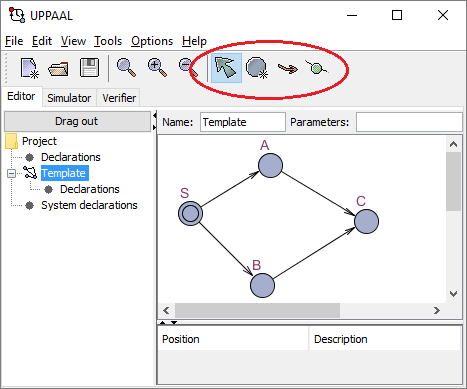
\includegraphics[scale=0.7]{img/uppaal_gui_small_editor_control.png}
			\end{figure}
		\end{column}
		
		\begin{column}{0.3\textwidth}
			\begin{itemize}
				\item Name: Template (default)
				\item Select
				\item Add location
				\item Add edge
				\item Add nail
				\item Syntax check (for global, local, system declarations)
			\end{itemize}
		\end{column}
	\end{columns}		
\end{frame}

\begin{frame}{Uppaal GUI - Simulator}
	\vspace{-5mm}
	\begin{columns}
		\begin{column}{0.8\textwidth}
			\begin{figure}[H]
				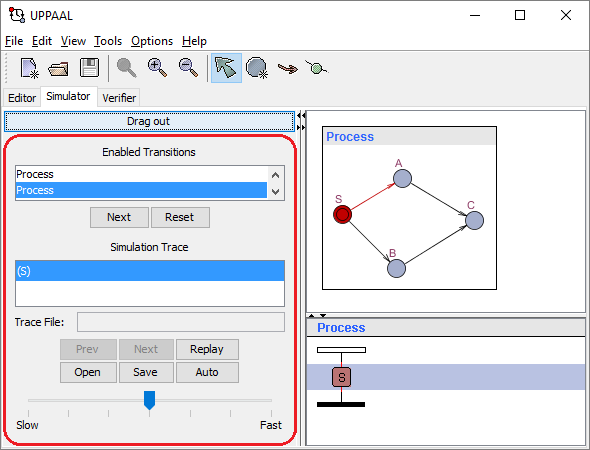
\includegraphics[scale=0.55]{img/uppaal_gui_small_simulation.png}
			\end{figure}
		\end{column}
		
		\begin{column}{0.35\textwidth}
			\begin{itemize}
				\item Select transition
				\item Track simulation
				\item Control (Prev/Next/Auto)
				\item Visualization
			\end{itemize}
		\end{column}
	\end{columns}		
\end{frame}

\begin{frame}{Uppaal GUI - Verifier}
	\vspace{-5mm}
	\begin{columns}
		\begin{column}{0.8\textwidth}
			\begin{figure}[H]
				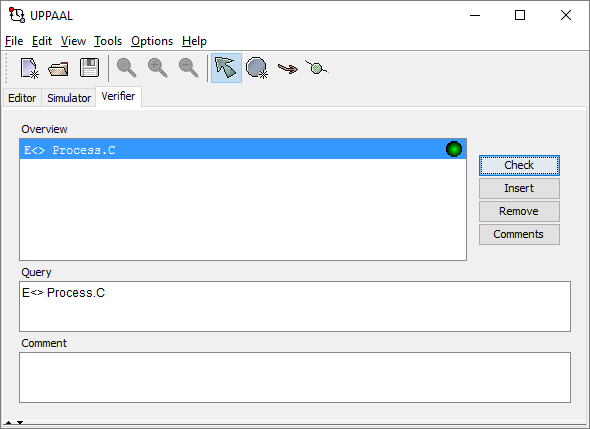
\includegraphics[scale=0.55]{img/uppaal_gui_small_verification.png}
			\end{figure}
		\end{column}
		
		\begin{column}{0.35\textwidth}
			\begin{itemize}
				\item Query editor
				\item Check query
				\item Overview
				\item Save/load
			\end{itemize}
		\end{column}
	\end{columns}		
\end{frame}

%%%%%%%%%%%%%%%%%%%%%%%%%%%%%%%%%%%%%%%%%%%%%%%%%%%%%%%%%%%%%%%%%%%%%%%%%%	
\subsection{Model structure}
%%%%%%%%%%%%%%%%%%%%%%%%%%%%%%%%%%%%%%%%%%%%%%%%%%%%%%%%%%%%%%%%%%%%%%%%%%
\begin{frame}{System/model/project}
%We build so called system/model/project.
	
	\begin{columns}
		\begin{column}{0.7\textwidth}
			Description of system consist of:	
			\begin{itemize}
				\item Concurrent process templates modelled using timed-automata (here \textit{P0} and \textit{P1});
				\item Local declarations for each process;
				\item Global declarations for whole system;
				\item System definition.
			\end{itemize}
		\end{column}
		
		\begin{column}{0.37\textwidth}
			\begin{figure}[H]
				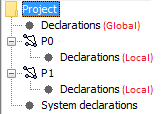
\includegraphics[scale=1]{img/uppaal_project.png}
			\end{figure}
		\end{column}
	\end{columns}
\end{frame}

\subsubsection{Processes}

\begin{frame}{Process/automata}
	
	Process is a timed-automata represent as diagram with states
	(called locations) and transitions between states (called edges). Timed-automata is finite state machine with time (clocks).\newline

	Each process has only one \textbf{initial location}.\newline
	
	Processes execute concurrently and they can be synchronized using channels.\newline
\end{frame}

\begin{frame}{Time/clocks}
	Time is continuous and the clocks measure time progress. \textbf{Time progress globally} and clocks values \textbf{increase at the same rate} for the whole system.\newline
	
	A clock is a special type of variable with domain being a set of non-negative real numbers. At system start, all clocks have value 0.\newline
	
	Using clocks we can specify:
	\begin{itemize}
		\item \textbf{Invariants} - upper bounds on timing, describes how long we can stay in given \textit{location} (e.g. \textit{x $<=$ 5});
		\item \textbf{Guard} - lower bound on timing, describes after what amount of time a \textit{transition} can be executed (e.g. \textit{x $>$ 2}).
	\end{itemize}
	
	We can test the value of clock using standard expressions or we can reset clock.
\end{frame}

\begin{frame}{Location/state (part I)}
	\begin{figure}[H]
		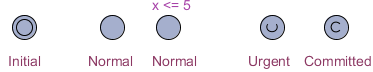
\includegraphics[scale=1]{img/uppaal_locations.png}
	\end{figure}
	
	Location represents state of the system. There are four types of locations:
	\begin{itemize}
		\item \textbf{Initial} (one for each process);
		\item \textbf{Normal} (with or without \textbf{invariants});
		\item \textbf{Urgent} (time cannot elapse in this location, so transition to another location must occur \textbf{immediately});
		\item \textbf{Committed} (they freeze time, if any process is in committed location then the next transition must involve and edge from one of the committed locations).
	\end{itemize}
\end{frame}

\begin{frame}{Edge/transition (part I)}
	An edge/transition connects two locations. Edges can have four types of annotations:
	
	\begin{itemize}
		\item \textbf{Selection} - binds a given identifier to a random value in a scope of current transition; allowed types: \textit{boundend integers}, \textit{scalar sets}; defined here identifiers will shadow local/global variables.
		\item \textbf{Guard} - transition is enabled only if guard's expression evaluates to \textbf{true} and consists of:
		\begin{itemize}
			\item Conjunction of simple conditions on clocks;
			\item Differences between clocks;
			\item Boolean expressions not involving clocks.
		\end{itemize}
		\item \textbf{Synchronization} - transition labelled with complementary actions (e.g. \textit{a!} and \textit{a?}) will synchronize over a common channel (here channel \textit{a})
	\end{itemize}

\end{frame}

\begin{frame}{Edge/transition (part II)}
	\begin{itemize}
		\item \textbf{Update} - evaluate given expression when transition occur.
	\end{itemize}	
	
	\begin{figure}[H]
		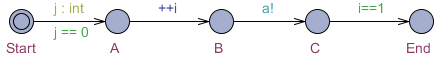
\includegraphics[scale=0.8]{img/uppaal_transitions.png}
	\end{figure}
	Example of transitions with annotations:
	\begin{itemize}
		\item Selection: \textit{j : int};
		\item Update: \textit{++i};
		\item Synchronization: \textit{a!};
		\item Guard: \textit{j==0}, \textit{i==1}.
	\end{itemize}
\end{frame}

\begin{frame}{Edge/transition (part III)}
	\vspace{-2mm}
	\begin{itemize}
		\item Without prior specification, \textbf{all transitions occur instantaneously} and do not take time (they have default guard which always evaluate to \textbf{true});
		\item When no further transition is possible we reach so called \textbf{deadlock state};
		\item Unspecified choice is called non-deterministic (look at figures below).
	\end{itemize}
	\vspace{-7mm}	
	\begin{columns}
		\begin{column}{.5\textwidth}
			\begin{figure}[H]
				\label{img:ndc}
				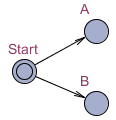
\includegraphics[scale=0.7]{img/uppaal_non_deterministic_choice.png}
				\caption{Non-deterministic choice.}
			\end{figure}
		\end{column}
		\begin{column}{.5\textwidth}
			\begin{figure}[H]
				\label{img:dc}
				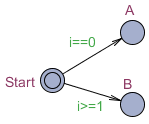
\includegraphics[scale=0.7]{img/uppaal_deterministic_choice.png}
				\caption{Deterministic choice.}
			\end{figure}
		\end{column}		
	\end{columns}
\end{frame}

\begin{frame}{Location/transition - a thing to remember}
	If not specified, \textit{locations} can wait \textbf{forever}, but \textit{transitions} will execute \textbf{immediately}.
\end{frame}

\begin{frame}{Parameters of process template}
	
	Template of a process can have input parameters with different pass semantics (C++ syntax \& semantic):
	
	\begin{itemize}
		\item \textbf{pass-by-value} (using local copy, e.g. \textit{int a})
		\item \textbf{pass-by-reference} (using original value, e.g. \textit{int\& a})
	\end{itemize}
	
	Clocks and channels should be pass-by-reference parameters.\newline
	
	Examples:
	\begin{itemize}
		\item \textit{P(clock \&x, bool bit)}
		\item \textit{Q(clock \&x, clock \&y, int i1, int \&i2, chan \&a, chan \&b)}
	\end{itemize}
	Creating such template: \textit{P0 = P(clock, true);}\newline
	
	This pass semantics are true also for functions' parameters.	
\end{frame}

\subsubsection{Declaration}

\begin{frame}{Declarations}
	Declarations can be global (in one place) or local (to a template). They mostly consist of programming statements and expressions with syntax similar to C++. Declarations mostly consist of:
	\begin{itemize}
		\item Clocks (e.g. \textit{clock x, y;})
		\item Bounded integers (e.g. \textit{int[0,100] a=5;})
		\item Channels (e.g. \textit{chan d; urgent chan e;})
		\item Arrays (e.g. \textit{int a[2][3] = \{\{1, 2, 3\}, \{4, 5, 6\}\}})
		\item Records (e.g. \textit{struct \{int a; clock c;\} S;})
		\item Types (e.g. \textit{typedef} keyword)
		\item Functions
	\end{itemize}
	Uppaal does not support enumerated types.
\end{frame}

\begin{frame}{Data types (part I)}
	We have four predefined data types:
	\begin{enumerate}
		\item Integer (\textit{int}) - default value range is $[-32768, 32767]$;
		\item Boolean (\textit{bool}) - \textbf{true} (1)/\textbf{false} (0) values;
		\item Clock (\textit{clock}) - non-negative real values;
		\item Channel (\textit{chan}) - with three subtypes: \textbf{normal}, \textbf{urgent} and/or \textbf{broadcast}.
	\end{enumerate}
\end{frame}

\begin{frame}{Data types (part II)}
	\begin{itemize}
		\item We can have \textbf{constant} integers, booleans and arrays/records over integers and booleans (e.g. \textit{const int i = 1;}).
		\item We can have these variables marked as \textbf{meta}, so that they are stored in the state vector, but they are not part of state. Meta variables won't affect state a space exploration \\ (e.g. \textit{meta bool edgeVisited[N\_EDGES];} or for swapping variables).
		\item Variable assigned with a value outside of its domain generates ``run-time error''.
	\end{itemize}

\end{frame}

\begin{frame}[fragile]{Functions}
	Almost identical to C++ like functions. Some simple examples:
	\small
	\begin{verbatim}
		void initialize(int& a[10]) {
		    for (i : int[0,9]) {
		        a[i] = i;
		    }
		}
	\end{verbatim}
	
	\begin{verbatim}
	void swap(int &a, int &b) {
	    int c = a;
	    a = b;
	    b = c;
	}
	\end{verbatim}
	
\end{frame}

\begin{frame}[fragile]{System declaration}
	We can define here global variables, channels and functions. They are not accessible in process templates because they are defined before them.
	
	First we instantiate processes then we create system. Examples:
	
	\tiny{
	\begin{verbatim}
	process ProcA() {}
	process ProcB(int& x, bool b, int y) {}
	(...)
	// System declaration starts here!
	int x = 5;
	P0 = ProcA();
	P1 = ProcB(x, true, 15);
	// Partial instantiation
	Q(int& z) = ProcB(x, true, z);
	P2 = Q(10);
	
	system P0, P1, P2;
	// Or with priorities
	system P0 < P1 < P2;
	\end{verbatim}}
\end{frame}

\begin{frame}{Synchronization and channels}
	In Uppaal there is a hand-shaking synchronization: two processes take a transition at the same time, only when one will have an \textit{\textbf{a!}} (emit) and the other an \textit{\textbf{a?}} (receive), where \textit{\textbf{a}} is a channel used.\newline
	
	First the \textbf{update expression} is executed on transition synchronized on \textit{\textbf{a!}} then on other transition annotated with \textit{\textbf{a?}}.
	
	We have three types of channels:
	\begin{enumerate}
		\item \textbf{Binary/Normal};
		\item \textbf{Broadcast} - allows 1-to-many synchronization.
		\item \textbf{Urgent} - source state can't delay triggering a synchronized transition, it must be triggered instantly when possible; clock conditions on these transitions are not allowed;
	\end{enumerate}
	
	There is no value passing through the channels.
	
\end{frame}

\begin{frame}[fragile]{Priorities}
	Channels and processes can have specified priorities. Examples for channels:
	
	\begin{verbatim}
		chan priority a, b < default < c;
	\end{verbatim}
	
	Processes priorities are specified in system declaration:
	
	\begin{verbatim}
		system P0 < P1 < P2, P3;
	\end{verbatim}
\end{frame}

\subsubsection{Queries}

\begin{frame}{Queries (part IA)}	
	Query describe a property expressed as temporal logic formula, that may or may not hold for a given model. The Verifier can establish whether the query is \textbf{satisfied} or \textbf{not}.\newline
	Basic queries:
	\begin{itemize}
		\item \textit{A[] p} : for all paths \textit{p} \textbf{always holds};
		\item \textit{E[] p} : there exists a path where \textit{p} \textbf{always holds};		
		\item \textit{A$<>$ p} : for all paths \textit{p} will \textbf{eventually hold};
		\item \textit{E$<>$ p} : there exists a path where \textit{p} \textbf{eventually holds};
		\item \textit{p --$>$ q} : whenever p holds q will eventually hold.

	\end{itemize}
	
	Simple queries are in form of e.g \textit{A[] p} where \textit{p} is an expression build from \textbf{boolean combination} of \textbf{atomic propositions}.
\end{frame}

\begin{frame}{Queries (part IB)}
	Property equivalences:
	\begin{tabular}{|c|c|c|}
		\hline \textbf{Name} & \textbf{Property} &\textbf{ Equivalent to }\\ 
		\hline Possibly & \textit{E$<>$ p} &  \\ 
		\hline Invariantly & \textit{A[] p}  & \textit{not E$<>$ not p} \\ 
		\hline Potentially always &	\textit{E[] p}  &  \\ 
		\hline Eventually & \textit{A$<>$ p} & \textit{not E[] not p} \\ 
		\hline Leads to & \textit{p --$>$ q} & \textit{A[] (p imply A$<>$ q)} \\ 
		\hline 
	\end{tabular} 
\end{frame}

\begin{frame}{Queries (part II)}
	The simplest atomic proposition can be of the form \textit{P0.C}, where \textit{P0} is an automaton and \textit{C} is a location. Such a proposition is \textbf{true} if process \textit{P0} is in location \textit{C}.\newline
	
	\begin{tabular}{|c|c|c|}
		\hline \textbf{Expression} & \textbf{Name} & \textbf{True when...} \\ 
		\hline $e\text{ }\&\&\text{ }f$ & and & $e$ and $f$ evaluate to \textbf{true}	 \\ 
		\hline $e\text{ }||\text{ }f$ & or & $e$ or $f$ evaluate to \textbf{true} \\ 
		\hline $e\text{ }==\text{ }f$ & equality & $e$ and $f$ evaluate to the same value \\ 
		\hline $e\text{ }imply\text{ }f$ & implication & $e$ evaluate to \textbf{false} or $f$ evaluate to \textbf{true}\\ 
		\hline $e\text{ }not\text{ }f$ & negation & $e$ evaluates to \textbf{false} \\ 
		\hline 
	\end{tabular} 

\end{frame}

\begin{frame}{Queries (part III)}
	\begin{itemize}
		\item $A[] \text{ not deadlock}$
		\item $E<> \text{Process\_1.C}$
		\item $E<> (\text{Process\_1.C } \&\& \text{ Process\_2.C})$
		\item $A[] \text{ now } >= \text{ 200 imply }$
		$(\text{Belt.end } \&\& \text{ Jobber1.begin } \&\& \text{Jobber2.begin})$
		\item $A[] \text{ Obs.taken imply } (x>=2 \text{ and } x<=3)$
		\item $E<> \text{ Obs.idle and } x>2$
		\item $A[] \text{ Obs.idle imply } x<=3$
		
	\end{itemize}
\end{frame}

\begin{frame}{Reasoning (part I)}
	The checking engine do an exhaustive search	that covers all possible dynamic behaviours of the system in order to check specification properties described in form of queries.\newline


	``More precisely, the engine uses \textbf{on-the-fly verification} combined with a \textbf{symbolic technique reducing the verification problem} to that of \textbf{solving simple constraint systems} [YPD94, LPY95]. The verifier checks for simple invariants and reachability properties for efficiency reasons. Other properties may be checked by using testing automata [JLS96] or the decorated system with debugging	information [LPY97].'' (\textit{Uppaal 4.0 : Small Tutorial})
	
\end{frame}

\begin{frame}{Reasoning (part II)}
	Uppaal provide a concrete example illustrating why the property holds (for \textit{E$<>$} properties) or not (for \textit{A[]} properties, so called: \textit{counterexample}).\newline
		
	In the case of \textit{E$<>$} properties that do not hold, or \textit{A[]} properties that hold, Uppaal can only report that it exhaustively checked all the reachable states of the model and didn't find anything.\newline
	
	It is worth to point out that model checker engine can run in \textbf{server mode} on a more powerful, dedicated machine.
\end{frame}


\begin{frame}{Saving data}
	We can save various types of data:
	
	\begin{itemize}
		\item Model/system - \textit{*.xml} file;
		\item Queries - \textit{*.q} file;
		\item Traces (binary) - \textit{*.xtr} file.
	\end{itemize}
\end{frame}

\begin{frame}{Keeping models manageable}
	\begin{itemize}
		\item \textbf{Committed locations} - reduce significantly the state space, but on the other hand they can take away relevant states;
		\item \textbf{Variables with ranges} - use small amount of variables with the shortest value ranges possible;
		\item \textbf{Minimum amount of clocks} - has an important impact on the complexity of the model.
	\end{itemize}
\end{frame}

%%%%%%%%%%%%%%%%%%%%%%%%%%%%%%%%%%%%%%%%%%%%%%%%%%%%%%%%%%%%%%%%%%%%%%%%%%	
\section{Example}
%%%%%%%%%%%%%%%%%%%%%%%%%%%%%%%%%%%%%%%%%%%%%%%%%%%%%%%%%%%%%%%%%%%%%%%%%%

\begin{frame}{Examples}
	\begin{enumerate}
		\item Non-deterministic process with synchronization (with one and two loops);
		\item Taken-idle with loop;
		\item Production line.
	\end{enumerate}
\end{frame}

%%%%%%%%%%%%%%%%%%%%%%%%%%%%%%%%%%%%%%%%%%%%%%%%%%%%%%%%%%%%%%%%%%%%%%%%%%	
\section{Bibliography}
%%%%%%%%%%%%%%%%%%%%%%%%%%%%%%%%%%%%%%%%%%%%%%%%%%%%%%%%%%%%%%%%%%%%%%%%%%

\begin{frame}
	\begin{itemize}
		\item F.W. Vaandrager. \textit{``A First Introduction to Uppaal''} In J. Tretmans, editor. Quasimodo Handbook. To appear.
		\item \textit{Uppaal 4.0: Small Tutorial. A short description of the tool as well as some examples.}
		\item \textit{Uppaal Help/Documentation}. Built-in. Uppaal 4.0.14, May 2014.
	\end{itemize}
\end{frame}

\end{document}
